\documentclass{article}
\usepackage{helvet}
\renewcommand{\familydefault}{\sfdefault}
\usepackage{enumitem,amssymb}
\usepackage{lipsum} % for filler text
\usepackage{geometry}
\geometry{
	paperwidth=5.5in,
	paperheight=8.5in,
	top=0.25in,
	bottom=0.5in,
	left=0.25in,
	right=0.25in,
	footskip=20pt  % Reserve space for footer
}
\usepackage{qrcode}
\newlist{todolist}{itemize}{2}
\setlist[todolist]{label=$\square$}
\usepackage{easylist}
\usepackage{fancyhdr}

\fancyfoot{} % clear all footer fields

\fancyfoot[C]{How To Build A Durable Community vVERSIONNUMBER} % other info in "inner" position of footer line
\usepackage{hyperref}
\usepackage{tikz}
\usepackage{rotating}
\usepackage{dashbox}
\usepackage{graphicx}
\usepackage{eso-pic} % allows background placement
\pagestyle{fancy}
\usepackage{sectsty}
\sectionfont{\centering}

% Set the value
\newlength{\mylen}
\setlength{\mylen}{0.25in}
\usepackage{lmodern}
\usepackage{tikz}
\usetikzlibrary{shapes.geometric, arrows.meta, positioning}
\input{src/how-to-consensus-zine/flow-chart-only.tex}%

\input{helper}

\input{MakerCheck.tex}%

\usepackage{multicol}


\usepackage{atbegshi}
\AtBeginShipout{\AddCornerImage}
\usepackage{amssymb}  % in preamble

% Define a convenient command (optional but handy)
\newcommand{\checkbox}{$\square$}

\usepackage{titlesec}
\titleformat{\section}{\normalfont\fontsize{9}{11}\bfseries\centering}{\thesection}{1em}{}
\titleformat{\subsection}{\normalfont\fontsize{8}{10}\bfseries}{\thesubsection}{1em}{}
\begin{document}
	
	\fontsize{8}{8}\selectfont

	\input{cover}	
	
	\pagebreak
	
	\input{read}
	
	\pagebreak
	
 	\input{durable.tex}
  
	\pagebreak
	
 	\input{common.tex}	
	
	\pagebreak
	
	\input{why.tex}	
	
	\pagebreak
	
	\input{consensus}

	\pagebreak
	
	
	\begin{center}
		\consensusflowchart{0.9}{\large}
	\end{center}
	
	\linedpagetwo
	
	\vspace{1cm}
	\pagebreak

		\section{What is Property?}
\subsection{ Legal Definitions}

This category is referred to as "Private Property" and is a collection of a few distinct rights. These are the rights enforced and recognized by law. 

\begin{enumerate}
	
	\item \textbf{Usufruct} - the right to use and receive the value from a piece of the physical world. An example would be public parks, we have the right to use them, but not the right to sell or destroy it.
	
	\item \textbf{Destruction} - the right to destroy a piece of the physical world. This can be as simple as eating an apple you own, but also the right to destroy anything defined as personal property. This right is constrained by laws such as historic preservation laws. 
	
	\item \textbf{Exclusion} -  the right to exclude others. You can demand someone leave private property, and are granted the right to have police use force to compel compliance. 
	
	\item \textbf{Transfer} - the right to transfer the property right to another individual or entity. This is your right to sell or give away ownership of some personal property. 
	
	\item \textbf{Increase (rent)} - the right to receive economic rents. These can be rent, interest, dividends and capital gains. 
\end{enumerate}



\subsection{Categories in a Commons}

Within a Commons, once the external entity has been assigned Private Property rights within the law, then that "bubble" can ascribe the rights according to its own rules. The commons can allocate areas of the pieces of the physical world that it manages (the clearly defined boundaries). The allocations can be for consumed aspects (the increase), it can be to assign use terms (Usufruct). Those who manage a commons determine to what degree exclusion and destruction are used within the commons.


\subsection{Personal Property} The items or space that is exclusively assigned along the legal definition. These can be either private property that came with someone into the commons, or can be the appropriators allocated share of some bounty. 


\subsection{Commons Space} This is the piece of the physical world that may have Usufruct allocated to members, or the public. These generally have the right of destruction held within the commons (for repairs and upgrades). The right to exclude is also held by the commons itself to determine if and when people can or will be excluded. 

\subsection{Public Space} This is space held by the state that assigned property rights. Examples would be the roads, infrastructure and public lands such as parks. The public might be granted usufruct rights, but not transfer, destruction, exclusion or increase. 

	\pagebreak

	\input{own}	
	
	\pagebreak
	
	\linedpagetwo
	
	\linedpagetwo
	
	\pagebreak
	
	\input{how}
	
	
	\pagebreak
	
	
% Add background image
\AddToShipoutPictureBG*{%
	\AtPageLowerLeft{%
		\raisebox{7mm}{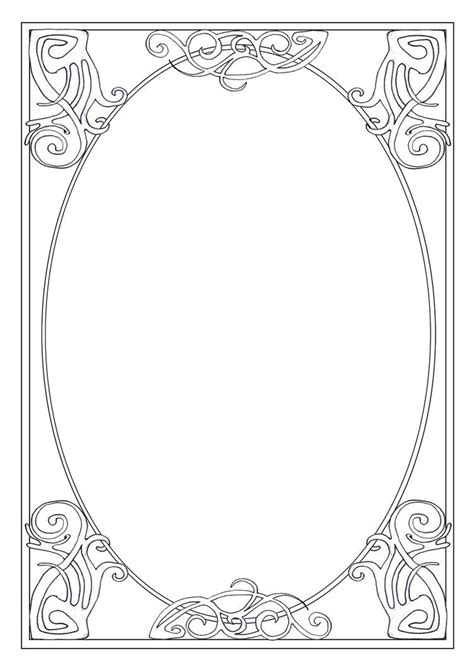
\includegraphics[width=\paperwidth,height=\dimexpr\paperheight-10mm\relax]{src/how-to-consensus-zine/mucha.png}}%
	}%
}

\vspace*{\fill}
{\centering 

	\begin{center}
		\begin{minipage}{0.75\textwidth}
			\centering
			\Large ``The ultimate hidden truth of the world is that it is something that we make,
			
			 and could just as easily make differently,''
			 
			\vspace{1em} % Space between title and subtitle
			
			 $\sim$ David Graeber
		\end{minipage}
	\end{center}
}
\vspace*{\fill}
	
\end{document}
